\documentclass{article}

\usepackage{spconf,amsmath,amssymb,graphicx,hyperref}
\usepackage[utf8]{inputenc}
\usepackage{float}
\usepackage[table]{xcolor}
\usepackage{color}
\definecolor{win}{RGB}{0, 150, 0} % Green
\definecolor{loss}{RGB}{200, 0, 0} % Red
\usepackage{subcaption}
\usepackage{etoolbox}
\usepackage[scaled=.7]{beramono}
\usepackage{booktabs}
\usepackage{siunitx}

\AtBeginEnvironment{thebibliography}{
  \fontsize{8pt}{8.8pt}\selectfont
  \setlength{\itemsep}{0pt}
  \setlength{\parskip}{0pt}
}



\title{Unifying Speech and Language Through Continuous Dual-Fusion for Medium-Resource Languages: The Cases of Hungarian and Greek}

\name{\textit{Christos Siargkas},
    \textit{Nikos Ellinas },
    \textit{Georgios Vamvoukakis},
    \textit{Georgios Dimitriou}, \\
    \textit{Alexandra Vioni},
    \textit{Panagiotis Kakoulidis},
    \textit{Konstantinos Markopoulos},
    \textit{Georgios Vardaxoglou}, \\
    \textit{Jeasung Lee},
    \textit{Sangshin Oh},
    \textit{Gunu Jho},
    \textit{Inchul Hwang},
    \textit{Pirros Tsiakoulis},
    \textit{Aimilios Chalamandaris}}

\address{Samsung}

\begin{document}
\ninept
\maketitle

\begin{abstract}
    In medium-resource languages like Hungarian and Greek, Automatic Speech Recognition (ASR) suffers from scarce paired acoustic data, whereas abundant text data can be leveraged via Large Language Model (LLM) priors. To compensate for this acoustic deficit, we propose a Dual-Fusion architecture that conditions ASR decoding on continuous acoustic information at both the prompt level and inside the LLM's intermediate layers. Our model bridges a frozen acoustic encoder with pre-trained LLMs via both prompt-level embeddings and deep, continuous-space alignment across multiple intermediate decoder layers. To actively control the semantic-acoustic trade-off, our methodology introduces asymmetric downsampling to preserve fine phonetic boundaries, multi-layer gated cross-attention, attention-weighted layer-wise fusion of the acoustic encoder's hidden states, and target text perturbation. Evaluated on diverse Hungarian and Greek datasets, our framework reduces Word Error Rate (WER) compared to both standalone acoustic decoders and acoustic-linguistic models like VoxKrikri, demonstrating consistent performance improvements across both languages.
\end{abstract}

\begin{keywords}
    Automatic Speech Recognition,
    Speech LLMs,
    Continuous Fusion,
    Medium-Resource ASR,
    Multimodal Alignment
\end{keywords}

\begin{figure*}[t]
    \hspace{-0.8cm}
    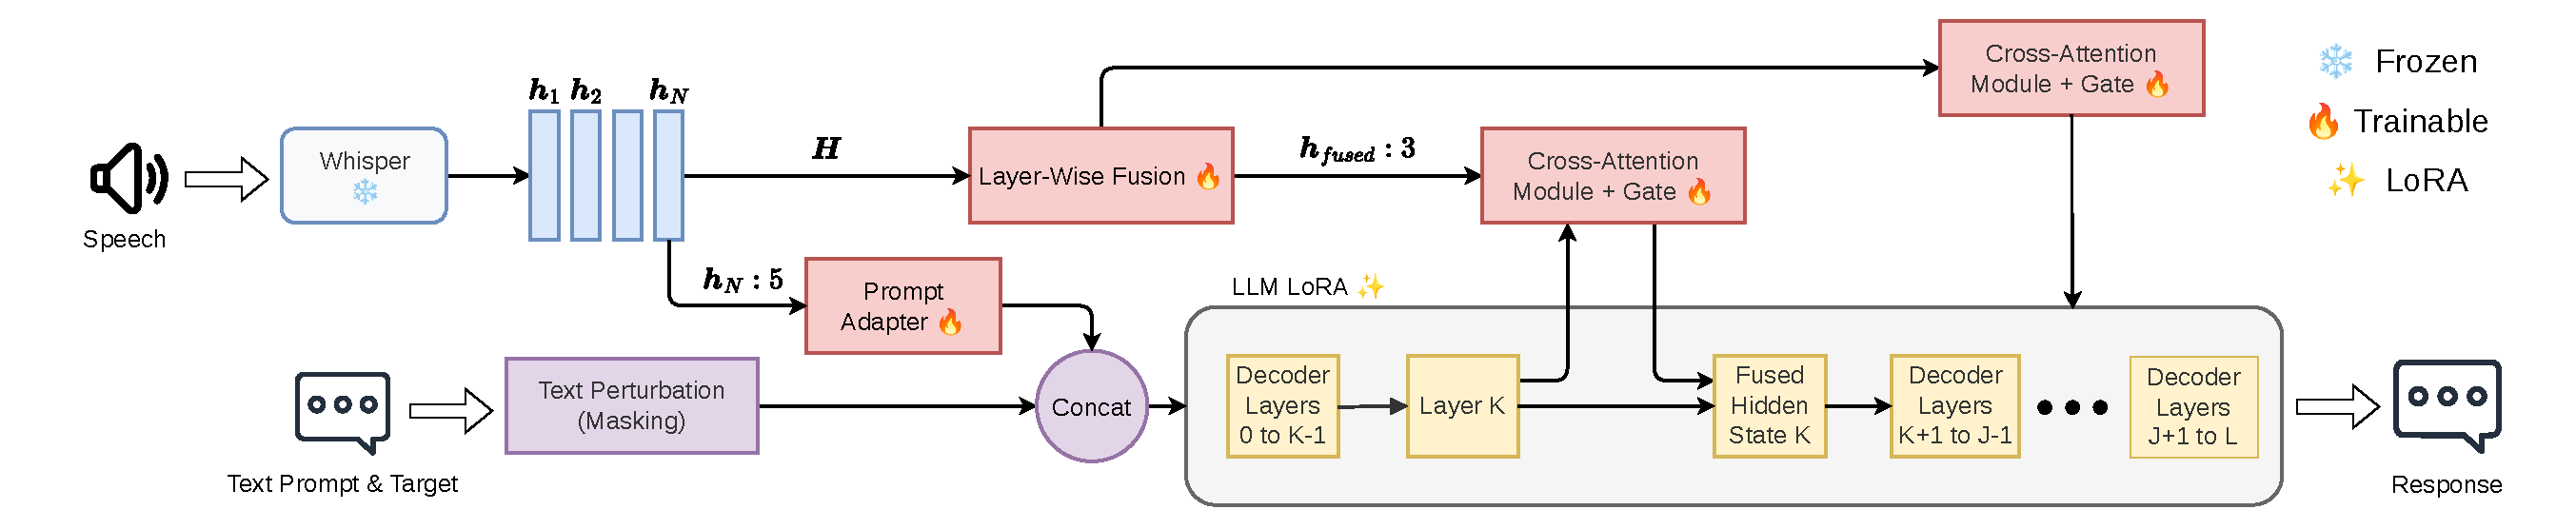
\includegraphics[height=115pt,keepaspectratio]{dual_fusion_architecture.drawio}
    \caption{
    Proposed Continuous Dual-Fusion ASR architecture: The speech instances are first processed by a frozen Whisper acoustic encoder, producing the acoustic hidden states $\boldsymbol{H} = \{\boldsymbol{h}_1 \dots \boldsymbol{h}_N\}$. These states are processed in parallel by two distinct fusion pathways to bridge them into the LLM embedding space. In the prompt-level path, the final acoustic state ($\boldsymbol{h}_N$) with dimensions $T \times D$ is downsampled by a factor of $k = 5$ and projected into the LLM space as prefix tokens of dimension $\lfloor{ T / 5}\rfloor \times D_{LLM}$ via an MLP adapter. Concurrently, in the cross-attention path, all encoder states $\boldsymbol{H}$ undergo Layer-Wise Fusion and Conv1D downsampling by a finer factor of $k = 3$ to form a phonetically rich acoustic representations of dimension $\lfloor{ T / 3}\rfloor \times D$. The LoRA-adapted LLM decoder follows; it processes the concatenated acoustic and text tokens, while aggregating the continuous acoustic representations via Gated Cross-Attention modules at multiple intermediate layers.
    }
    \label{fig:model_architecture}
\end{figure*}

\section{Introduction}
\label{sec:intro}
\noindent
Automatic Speech Recognition (ASR) has advanced significantly with robust end-to-end models like Whisper~\cite{radford2022robustspeechrecognitionlargescale} and data-efficient architectures like Canary~\cite{sekoyan2025canary1bv2parakeettdt06bv3efficient}, achieving state-of-the-art multilingual performance. However, these systems often degrade on medium-resource, morphologically complex languages such as Hungarian and Greek. We hypothesize this drop stems not solely from acoustic feature extraction, but partly from orthographic and morphological errors caused by a lack of deep, language-specific linguistic priors, consistent with evidence that external language models can improve low-resource ASR~\cite{dezuazo2025whisperlmimprovingasrmodels}.

To bridge this gap, recent research couples pre-trained acoustic encoders with Large Language Models (LLMs) in Speech-Language Models (SLMs)~\cite{fong2026speechllmslowresourcescenarios}, broadly following two integration strategies~\cite{chen2024bestow}: prompt-level approaches that prepend compressed acoustic embeddings as pseudo-text tokens, and cross-attention approaches that let text states attend to acoustic representations at intermediate layers. Early prompt-level strategies minimized architectural complexity: the SLAM-ASR framework~\cite{ma2024embarrassinglysimpleapproachllm} showed that a simple, trainable linear projector connecting a frozen encoder like Whisper to a frozen LLM yields competitive ASR. SALMONN~\cite{tang2024salmonngenerichearingabilities} extended this with a learned Q-Former to bridge audio embeddings into the LLM space. We hypothesize that the rigid temporal pooling used by such prompt-only connectors risks destroying micro-phonetic boundaries required for highly inflected languages; consistent with this concern, SLAM-ASR degrades under domain shift and acoustic perturbations~\cite{kumar2025performanceevaluationslamasrgood}.

For deeper semantic integration, cross-attention fusion was explored. The Whispering LLaMA framework~\cite{Radhakrishnan_2023} pioneered cross-modal generative error correction by integrating Whisper's audio embeddings directly into the LLM via cross-attention adapters. A comparative connector study~\cite{yu2023connectingspeechencoderlarge} reports that multi-head cross-attention, despite higher parameter cost than linear projectors, can yield better representational alignment than simple connectors. Furthermore, Whisper-Flamingo~\cite{rouditchenko2024whisperflamingointegratingvisualfeatures} established the efficacy of gated cross-attention to interleave frozen text blocks with continuous multimodal inputs, ensuring stable generation. In the speech domain, VoxKrikri~\cite{damianos2025voxkrikriunifyingspeechlanguage} operates fully within a continuous latent space, fusing Whisper's hidden decoder states with an LLM's textual representations at a single selected layer, showing that intermediate layer injection yields robust cross-modal alignment for Greek.
%TODO make a mention on a hungarian asr system {mihajlik-etal-2024-spoken}

A related question is which encoder representations to expose. Rather than passing only the final hidden state, SUPERB~\cite{yang2021superbspeechprocessinguniversal} established that different layers of a self-supervised speech encoder carry different phonetic and semantic information; follow-up work~\cite{chiu24_interspeech} shows learned weighted combination over all encoder layers can outperform single-layer extraction, and more recent work replaces static weights with input-dependent attention, e.g.\ Adaptive Layer Attention~\cite{tripathi2025listenliketeachermitigating} and TASLA~\cite{hsu2025taslatextalignedspeechtokens}. Finally, fused acoustic-LLM decoders often suffer the ``lazy LLM'' problem, ignoring acoustic information in favor of the text prior. We counter this with word dropout~\cite{bowman2016}, a remedy for VAE posterior collapse: masking target-history tokens during teacher forcing weakens access to clean linguistic context. This is related to, but distinct from, inference-time textual perturbation against multimodal-LLM hallucination~\cite{jia2026decodingperturbationmitigatingmllm}.

Building on these findings, we propose a Dual-Fusion architecture that couples a frozen Whisper encoder with language-specialized LLM backbones for Hungarian and Greek, combining: (i) a \textit{Dual-Fusion} strategy feeding acoustic information at both the prompt level and via cross-attention, with decoupled downsampling factors; (ii) \textit{multiple injection layers} with \textit{layer-wise fusion} of all Whisper encoder layers rather than only the final state; (iii) \textit{gated cross-attention} scaling injected context with a learnable $\tanh$ gate; and (iv) \textit{text perturbation}, substituting random tokens in the teacher-forced target sequence. We are not aware of a prior system that combines these within a single continuous, audio-conditioned architecture; we study whether doing so improves performance for both Hungarian and Greek, two typologically distinct medium-resource languages, and report a component-wise ablation (Section~\ref{subsec:ablation}). Evaluated on multiple Hungarian and Greek corpora against standalone Whisper and VoxKrikri, our Dual-Fusion models yield consistent Word Error Rate reductions across both languages.

\section{Methodology}

\noindent
The methodology couples a frozen Whisper encoder with a language-specific LLM (Racka-4B for Hungarian, Llama-Krikri-8B-Instruct for Greek) through prompt-level conditioning and intermediate cross-attention. An overview is given in Fig. \ref{fig:model_architecture}.

\subsection{Dual Fusion Strategy}
\noindent
To bridge the temporal mismatch between high-frequency acoustic frames and dense semantic tokens, we deploy asymmetric downsampling. In the \emph{prompt path}, the final Whisper encoder state $\boldsymbol{h}_N \in \mathbb{R}^{T \times D}$ is passed through a $\mathrm{reshape}$ operator to yield the downsampled state $\tilde{\boldsymbol{h}}_N \in \mathbb{R}^{\lfloor T / 5 \rfloor \times 5D}$.  A two-layer MLP then projects these downsampled representations into the LLM's embedding space, yielding the continuous acoustic tokens $\boldsymbol{S}_{prompt} \in \mathbb{R}^{\lfloor T / 5 \rfloor \times D_{LLM}}$. These are then concatenated into the LLM's input sequence as prefix tokens:
$$\mathrm{embed}(\text{prefix}) \,\Vert{}\, \boldsymbol{S}_{prompt} \,\Vert{}\, \mathrm{embed}(\text{text})$$
Crucially, this coarser downsampling factor ($k=5$, 100ms resolution) prevents quadratic computational bloat in the LLM's global self-attention sequence.
Conversely, the \emph{cross-attention path} injects speech-derived representations at selected layers using a finer Conv1D downsampler ($k=3$, 60ms resolution). This preserves the micro-phonetic boundaries essential for highly inflected languages—specifically, rapid Hungarian agglutinative suffixes and unstressed Greek vowel transitions. Maintaining this denser resolution is computationally viable because it strictly localizes to cross-attention operations without expanding the LLM's global sequence length. Ablations (Section~\ref{subsec:ablation}) confirm $k=3$ balances the model's performance against the prohibitive cost of $k=1$.


\subsection{Multiple Injection Layers as Persistent Acoustic Memory}
\label{subsec:multiple_injection}
\noindent
Rather than injecting at a single depth like VoxKrikri, we inject cross-attention simultaneously at three intermediate decoder blocks targeted at roughly 30\%, 60\%, and 90\% relative depth (blocks $[10, 20, 30]$ of 32 for KriKri, and $[15, 25, 35]$ of 36 for Racka). Repeated injection maintains a persistent acoustic memory, re-grounding generation instead of drifting toward pure language-model continuation.

\subsection{Layer-Wise Fusion of Acoustic Representations}
\noindent
We utilize all encoder hidden states $\{\boldsymbol{h}_1 \, \boldsymbol{h}_2 \cdots \, \boldsymbol{h}_N\}$, since lower states preserve phonetic detail and higher states carry semantic abstraction. A \textit{LayerWiseAttention} module mean-pools each state's representation over the time dimension and scores it with a shared MLP, producing an \emph{utterance-level} combination: $$\boldsymbol{h}_{fused}^{(j)} = \sum_{l=1}^{N} \alpha_{l}^{(j)}\, \boldsymbol{h}_{l}, \quad \alpha_{l}^{(j)} = \operatorname{softmax}_{l}\!\left(\boldsymbol{v}^{(j)\top}\tanh(\boldsymbol{W}^{(j)}\bar{\boldsymbol{h}}_{l})\right)$$

\subsection{Gated Cross-Attention}
\noindent
Injecting dense acoustic context directly into multiple intermediate layers of a pre-trained LLM risks overwhelming its established generative flow with unaligned, continuous signals from the very first training update. To ensure a stable adaptation process, we adopt the zero-initialized gating principle from Flamingo~\cite{alayrac2022flamingovisuallanguagemodel}. Each injection layer $j$ scales its cross-attention output with a single learnable scalar gate $g^{(j)}$: $$\tilde{\boldsymbol{h}}_{LLM} = \boldsymbol{h}_{LLM} + \tanh\!\left(g^{(j)}\right) \, \boldsymbol{C}_{audio}$$

\subsection{Text Perturbation}
\noindent
To counter the ``lazy LLM'' problem, where the decoder over-relies on the teacher-forced text prior and ignores the injected acoustic information, we introduce a dynamic text perturbation mechanism. During training, target-history tokens are independently masked (replaced by the padding token) with a probability of $p=10\%$. By stochastically masking the textual history during teacher forcing, the decoder is compelled to actively attend to the continuous acoustic representations to accurately predict the subsequent token. We set $p=10\%$ per the ablation in Section~\ref{subsec:ablation}.

\section{Experimental Setup}
\label{sec:experiments}

\subsection{Backbones and Injection Configuration}
\noindent
Both language configurations adopt the frozen Whisper-large-v3~\cite{radford2022robustspeechrecognitionlargescale} encoder (637M parameters). For Greek, the LLM backbone is Llama-KriKri-8B-Instruct~\cite{roussis2025krikriadvancingopenlarge} (8.2B base parameters, hidden dimension $D_{LLM} = 4096$, 32 decoder blocks); for Hungarian, elte-nlp/Racka-4B~\cite{csibi2026rackaefficienthungarianllm} (4.0B base parameters, $D_{LLM} = 2560$, 36 decoder blocks). The trainable bridge network dynamically scales to match each LLM's hidden dimension space. Specifically, the bridge consists of an MLP adapter (19M for Hungarian, 21.5M for Greek), a shared Conv1D downsampler (5M for both), cross-attention modules (59M for Hungarian, 132M for Greek), and a layer-fusion module (1M for both). This brings the total trainable parameters in Stage~1 to 84M for Hungarian and 160M for Greek, approximately 1.78\% of the full model size in both configurations. In Stage~2, low-rank adaptation adds 168M LoRA parameters on KriKri-8B and 133M on Racka-4B, while the Stage~1 bridge remains frozen.

\subsection{2-Stage LoRA Curriculum and Training Hyperparameters}
\noindent
In Stage 1, the LLM and Whisper encoder are fully frozen and only the bridge network is optimized, for 45k steps, with learning rate $10^{-4}$, an effective batch size of $64$ (per-device batch size $4$ with $4$ gradient-accumulation steps across $4$ GPUs), bf16 mixed precision, and the AdamW~\cite{loshchilov2019decoupledweightdecayregularization} optimizer under a cosine scheduler with warmup. In Stage 2, QLoRA~\cite{hu2021loralowrankadaptation, dettmers2023qloraefficientfinetuningquantizedllms} ($r=64, \alpha=128$) adapts the LLM for an additional 45k steps, targeting the attention projections and the gated-MLP up/down/gate projections; the bridge network trained in Stage 1 is frozen for the remainder of training so that LoRA adapts the LLM to the now-fixed acoustic interface rather than co-adapting with a still-moving bridge.

\subsection{Corpora}
\noindent
We evaluate on diverse corpora spanning formal, read, and spontaneous registers. For Greek, the datasets include Common Voice~\cite{ardila2020commonvoice}, FLEURS~\cite{conneau2022fleurs}, HParl~\cite{paraskevopoulos2023hparl}, TEDx~\cite{salesky2021mtedx}, and Logotypographia~\cite{digalakis2003logotypographia}. For Hungarian, we utilize Common Voice~\cite{ardila2020commonvoice}, FLEURS~\cite{conneau2022fleurs}, Speech Massive~\cite{lee2024speechmassive}, VoxPopuli~\cite{wang2021voxpopuli}, and Yodas~\cite{koluguri2025granaryspeechrecognitiontranslation}. The Hungarian training mixture also incorporates ``Internal-1'' and ``Internal-2'', comprising approx.\ 1,500 hours of conversational telephony and broadcast data. Each corpus is split into train/validation/test using the creators' official splits where provided, otherwise a 60/20/20 leave-subject-out split by speaker ID so that no speaker overlaps train and test. Because dataset sizes vary by orders of magnitude, batches are built via interleaved sampling across corpora (temperature $T = 1.2$).

%TODO which datasets are manually split?

\subsection{Preprocessing, Prompting, and Inference}
\noindent
Transcripts are normalized by removing non-spoken artifacts, such as speaker-tags and transcriber annotations, and by standardizing punctuation. We actively retain punctuation; this ensures the model learns to predict punctuation and syntactic boundaries directly from the acoustic signal and linguistic context. Utterances are conditioned on transcription style prompts: \texttt{[PROMPT\_CLEAN]} (clean transcript), \texttt{[PROMPT\_VERBATIM]} (word-for-word disfluencies retained), or \texttt{[PROMPT\_FORMAL]} (strictly formal). Each corpus is assigned the style matching its reference-transcription convention, applied consistently at training and inference. During training, Whisper's input features are also regularized with SpecAugment~\cite{park2019specaugment}. Inference uses beam search (beam width of 4) with a repetition penalty of $1.15$ and a 150-token maximum constraint.

\section{Results and Discussion}
We report Word Error Rate (WER), Character Error Rate (CER), and Normalized WER (N-WER), i.e.\ the error rate after stripping punctuation and casing (using Whisper's \texttt{BasicTextNormalizer}).
Because standard WER penalizes missing punctuation, strong results on both metrics indicate the architecture actively predicts syntactic boundaries from acoustic prosody.
However, we use N-WER as the primary comparative metric to align with the VoxKrikri baseline.

\subsection{Greek: Comparison Against Baselines}
\noindent
Table~\ref{tab:greek} compares against VoxKrikri (full-context, offline mode) and Whisper-v3 across five public Greek corpora. Our model outperforms VoxKrikri on Common Voice ($\Delta=-6.9$), HParl ($\Delta=-4.8$), and Logotypographia ($\Delta=-2.8$). FLEURS is the one corpus where VoxKrikri's simpler single-injection design wins ($\Delta=+0.6$), which qualitative analysis suggests stems from FLEURS's dense foreign named entities that our LLM's linguistic prior occasionally mis-transliterates (Section~\ref{subsec:limitations}).

\begin{table}[h]
\centering
\caption{Greek ASR performance. n-WER (\%) is the primary metric for comparison against baselines. Standard WER and CER are provided for our model for completeness.}
\label{tab:greek}
\footnotesize
\resizebox{\columnwidth}{!}{%
\begin{tabular}{l | c c c | c c}
\toprule
& \multicolumn{3}{c|}{\textbf{n-WER (\%)}} & \multicolumn{2}{c}{\textbf{Ours}} \\
\cmidrule(lr){2-4} \cmidrule(lr){5-6}
\textbf{Dataset} & \textbf{Ours} & \textbf{Vox (full)} & \textbf{Whisper} & \textbf{WER} & \textbf{CER} \\
\midrule
Common Voice(19h)~\cite{ardila2020commonvoice}            & \textbf{5.1} & 12.0 & 14.0 & 7.3 & 3.0 \\
FLEURS(12h)~\cite{conneau2022fleurs}                      & 9.9 & \textbf{9.3} & 11.0 & 10.9 & 4.8 \\
HParl(120h)~\cite{paraskevopoulos2023hparl}               & \textbf{8.2} & 13.0 & 17.0 & 8.2 & 4.7 \\
Logotypographia(61h)~\cite{digalakis2003logotypographia}  & \textbf{6.6} & 9.4   & 10.9 & 6.6 & 2.0 \\
TEDx(29h)~\cite{salesky2021mtedx}                         & 13.9 & --    & \textbf{12.3}  & 17.8 & 9.5 \\
\bottomrule
\end{tabular}%
}
\end{table}

%TODO fix results
%TODO check fair normalization baseline

\subsection{Hungarian: Comparison Against Baselines}
\noindent
Table~\ref{tab:hung} compares against Whisper large-v3 across all five public Hungarian corpora. We deliberately exclude the Whisper-Hu~\cite{trendency2024whisperlargev3hu} finetuned model due to disclosed test-set contamination on VoxPopuli, Common Voice, and Speech-Massive. Our model outperforms Whisper on four of five comparable corpora, with the largest margin on Common Voice ($\Delta = -7.1$). The sole loss is Yodas ($11.3$ vs.\ $6.2$, $\Delta = +5.1$), which likely reflects reference provenance rather than a real shortfall: Yodas transcripts are pseudo-labeled by faster-whisper-large-v3 itself, so comparing us to zero-shot Whisper on Whisper-generated references is close to self-referential evaluation.
To isolate architectural gains from the proprietary data advantage, Table~\ref{tab:public_data_ablation} reports a variant trained exclusively on public corpora. Without the 1,500-hour internal dataset the model degrades only marginally, retaining a strict advantage over Whisper on the four comparable datasets and confirming the efficacy of Dual-Fusion.

\begin{table}[h]
    \centering
    \caption{Hungarian ASR performance. n-WER (\%) is the primary metric for comparison against the baseline. Standard WER and CER are provided for our model for completeness.}
    \label{tab:hung}
    \footnotesize
    \resizebox{\columnwidth}{!}{%
    \begin{tabular}{l | c c | c c}
        \toprule
        & \multicolumn{2}{c|}{\textbf{n-WER (\%)}} & \multicolumn{2}{c}{\textbf{Ours}} \\
        \cmidrule(lr){2-3} \cmidrule(lr){4-5}
        \textbf{Dataset} & \textbf{Ours} & \textbf{Whisper} & \textbf{WER} & \textbf{CER} \\
        \midrule
        Common Voice(126h)~\cite{ardila2020commonvoice} & \textbf{6.0} & 13.1 & 7.4 & 2.0 \\
        FLEURS(14h)~\cite{conneau2022fleurs}            & \textbf{7.7} & 13.4 & 10.4 & 2.9 \\
        Speech Massive(6h)~\cite{lee2024speechmassive}  & \textbf{14.1} & 19.4 & 32.2 & 8.1 \\
        VoxPopuli(60h)~\cite{wang2021voxpopuli}         & \textbf{7.8} & 14.5 & 10.0 & 4.9 \\
        Yodas(114h)~\cite{li2023yodas}                  & 11.3 & \textbf{6.2} & 14.0 & 7.1 \\
        \bottomrule
    \end{tabular}%
    }
\end{table}

%TODO check fair normalization baseline
%TODO fix the table captions about $\Delta$

\begin{table}[h]
    \centering
    \caption{Impact of proprietary data on Hungarian n-WER (\%). \textbf{Ours (Full)} uses all data, while \textbf{Ours (Public)} is trained exclusively on public corpora. $\Delta$ indicates the absolute error rate degradation when internal datasets are removed.}
    \label{tab:public_data_ablation}
    \footnotesize
    \resizebox{\columnwidth}{!}{%
    \begin{tabular}{l | c c c c c}
        \toprule
        \textbf{Model Configuration} & \textbf{CV} & \textbf{FL} & \textbf{SM} & \textbf{VP} & \textbf{YD} \\
        \midrule
        Ours (Public) & 7.0 & 10.0 & 16.9 & 8.8 & 12.7 \\
        $\Delta$ vs.\ Ours (Full) & \textcolor{loss}{+1.0} & \textcolor{loss}{+2.3} & \textcolor{loss}{+2.8} & \textcolor{loss}{+1.0} & \textcolor{loss}{+1.4} \\
        \bottomrule
    \end{tabular}%
    }
    \\
    \vspace{6pt}
    \raggedright \scriptsize
    Note: CV (Common Voice), FL (FLEURS), SM (Speech Massive), VP (VoxPopuli), YD (Yodas)
\end{table}


\subsection{Ablation Study}
\label{subsec:ablation}
\noindent
To isolate component contributions without prohibitive training costs, we ablate on the validation set at 12k steps (Table~\ref{tab:ablation}), where the full model reaches $21.4$\% WER. Removing or altering any core component consistently degrades performance:
(i) removing the prefix audio tokens costs the most ($+3.3$), depriving the LLM's early layers of global acoustic context that, unlike cross-attention context, is visible to self-attention in every block from the first step;
(ii) using only the final encoder layer degrades WER by $1.8$, as intermediate layers retain phonetic detail~\cite{yang2021superbspeechprocessinguniversal}; static, utterance-independent layer weights recover part of this gap but still degrade by $+1.1$, showing that adapting the mixture per utterance brings a further gain;
(iii) removing the zero-initialized $\tanh$ gate ($+1.1$) injects randomly-initialized noise into the pre-trained LLM from the first update, whereas the gate ensures gradual integration of the acoustic signal;
(iv) masking 0\% of the target history costs $1.1$, as the model over-relies on text priors for subword completion, while excessive masking ($20$--$30$\%) destroys the linguistic context needed for clean inference;
(v) $k=5$ matches the prompt-path resolution and adds less temporal detail ($+0.4$), while $k=1$ gains only $0.2$ yet triples the key/value length of every cross-attention module, so $k=3$ offers the best accuracy--cost trade-off.

\begin{table}[h]
\centering
\caption{Ablation study for Hungarian on the validation set. $\Delta_W$ represents the WER degradation compared to the Full model.}
\label{tab:ablation}
\footnotesize
\resizebox{\columnwidth}{!}{%
\begin{tabular}{l | c c}
\toprule
\textbf{Configuration} & \textbf{WER (\%)} & \textbf{$\Delta_W$ vs.\ Full}\\
\midrule
Full model & 21.4 & -- \\
\midrule
Without Prompt Injection & 24.7 & \textcolor{loss}{+3.3} \\
\midrule
Without Layer-Wise Acoustic Fusion & 23.2 & \textcolor{loss}{+1.8} \\
With Input-Independent Layer Weights & 22.5 & \textcolor{loss}{+1.1} \\
\midrule
Without Gated Cross-Attention & \emph{22.5} & \textcolor{loss}{+1.1} \\
\midrule
Without Text Perturbation, $p=0\%$ & \emph{22.5} & \textcolor{loss}{+1.1} \\
With Text Perturbation, $p=20\%$& \emph{22.1} & \textcolor{loss}{+0.7} \\
With Text Perturbation, $p=30\%$& \emph{22.5} & \textcolor{loss}{+1.1} \\
\midrule
Cross-Attn Downsampling Factor $k=5$ & \emph{21.8} & \textcolor{loss}{+0.4} \\
Cross-Attn Downsampling Factor $k=1$ & \emph{21.2} & \textcolor{win}{-0.2} \\
\bottomrule
\end{tabular}%
}
\end{table}
%TODO mention Weak setup. The ablations are at 12k steps of Stage 1 (no LoRA), with one seed, Hungarian only, on an unspecified validation set.

\subsection{Cross-Attention Analysis}
\noindent
To substantiate the depth specialization hypothesized in Section~\ref{subsec:multiple_injection}, we measured attention entropy ($\bar{H}^$) and Pearson diagonality ($r$) over 1k random Common Voice samples across Racka's three injection layers $\lbrack15,25,35\rbrack$. As visualized in Fig.~\ref{fig:word_level_alignment}, each depth takes a distinct functional role: (i) layer 15 exhibits high entropy ($\bar{H} = 0.951$) and low diagonality ($r = 0.534$), for coarse salient event detection; (ii) layer 25 achieves sharp temporal focus, with the lowest entropy ($\bar{H} = 0.759$) and highest monotonic diagonality ($r = 0.887$), this precise grounding occurs at $\sim$69\% relative depth, corroborating independent findings for VoxKrikri~\cite{damianos2025voxkrikriunifyingspeechlanguage}; and (iii) layer 35 relaxes temporal tracking ($\bar{H} = 0.788$, $r = 0.704$), confirming its role in diffuse, non-monotonic global re-grounding.

\begin{figure}[h]
    \centering
    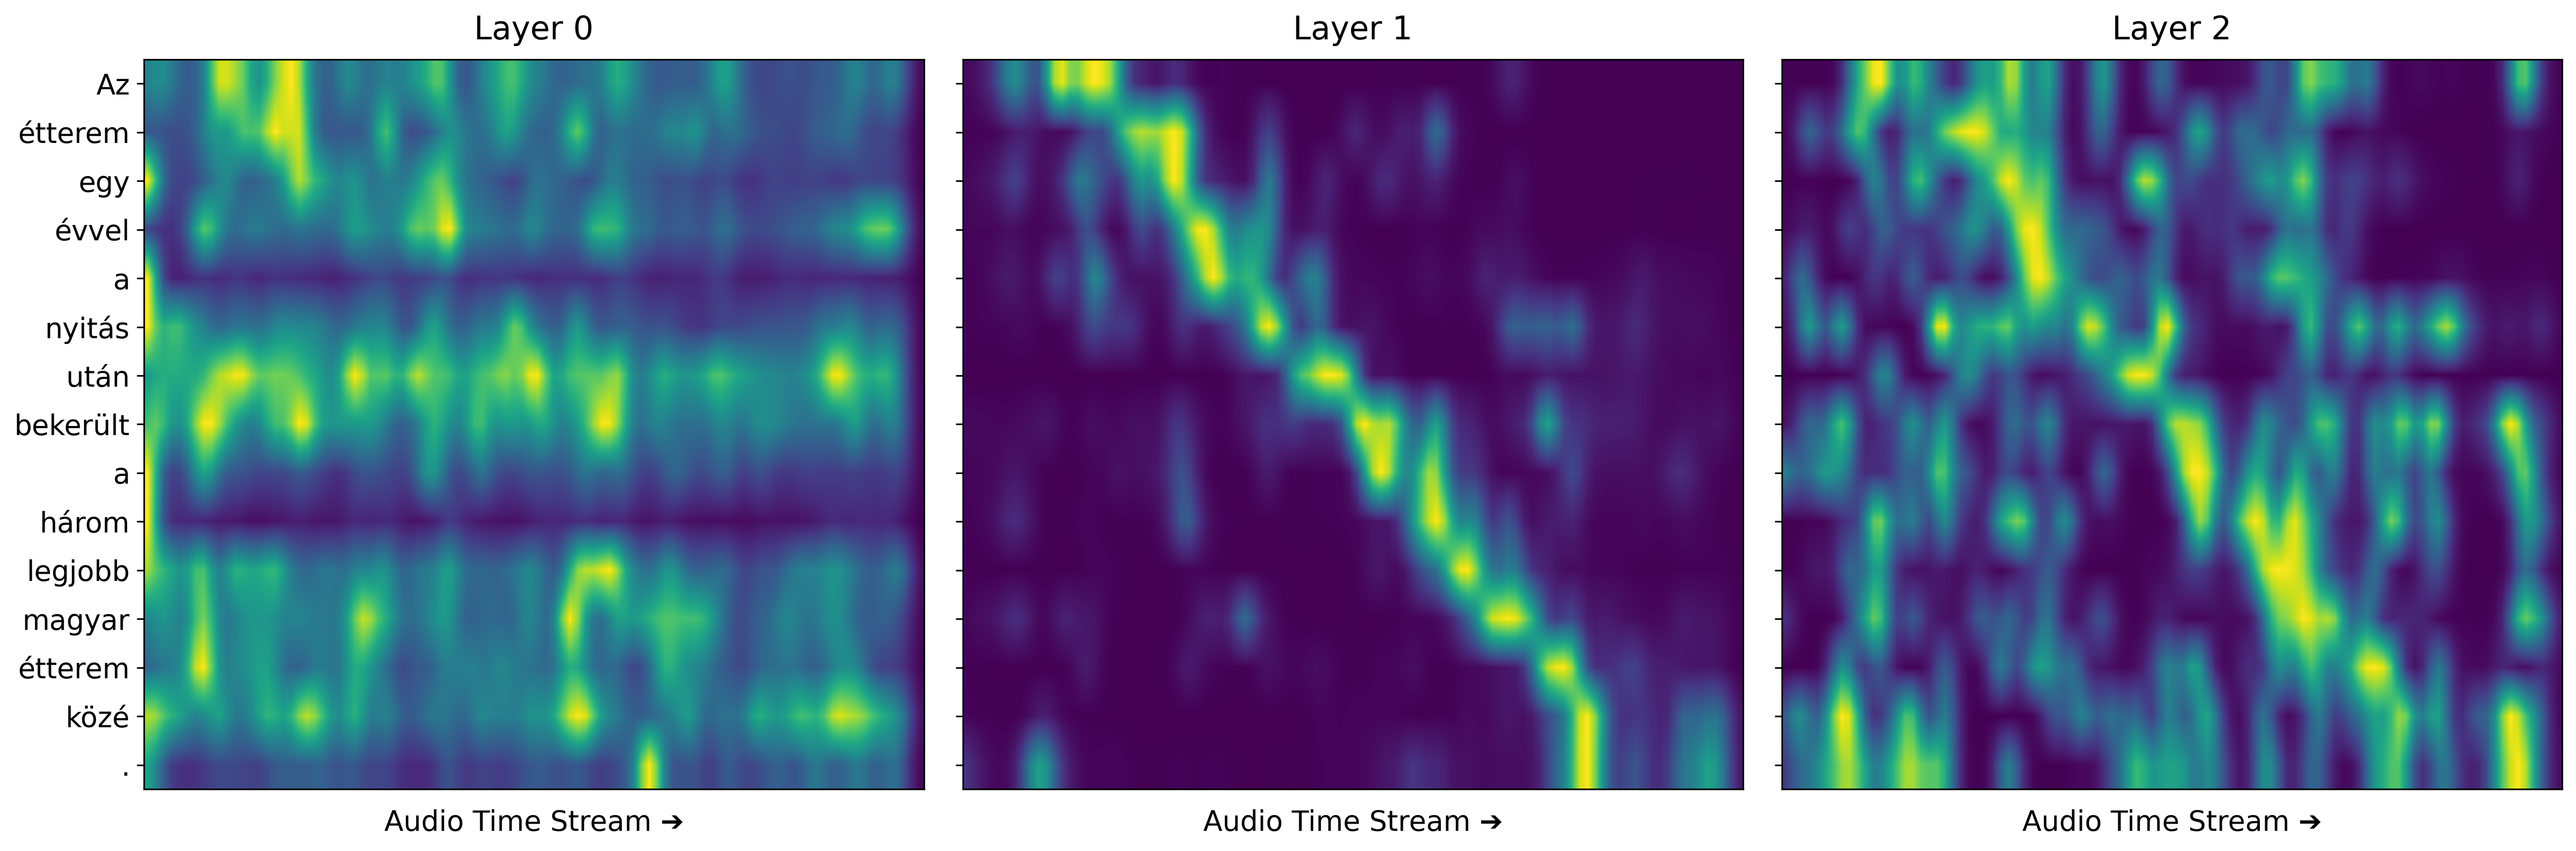
\includegraphics[height=82pt,keepaspectratio]{combined_word_alignment_common_voice(1).png}
    \caption{Word-level cross-attention alignment for a representative Hungarian test utterance across the three injection layers. Temporal tracking sharpens strictly in the middle layer (Layer 25).}
    \label{fig:word_level_alignment}
\end{figure}

\subsection{Limitations}
\label{subsec:limitations}
\noindent
Our qualitative analysis surfaces a recurring failure mode: because the fused LLM carries strong linguistic priors, it sometimes acts less like a verbatim transcriber and more like a ``copy editor'', silently dropping hesitation markers and disfluencies, normalizing colloquial contractions, occasionally completing thoughts on abruptly cut-off audio, and mis-transliterating foreign proper names. This inflates WER on disfluency-rich, verbatim-style corpora even when the output is fluent and faithful in meaning. Our evaluation is also limited to two medium-resource languages and a single frozen encoder (Whisper-large-v3); generalization to other languages, encoders, or truly low-resource settings remains untested.

\section{Conclusion \& Future Work}
\noindent
We presented a Continuous Dual-Fusion architecture coupling a frozen Whisper encoder with language-specialized LLMs for medium-resource ASR in Hungarian and Greek, using multi-layer gated cross-attention, layer-wise acoustic pooling, and text perturbation to ground generation in the acoustic signal without discarding linguistic priors. Across five Hungarian and five Greek corpora, our model reduces WER over standalone Whisper on all but one Hungarian corpus (Table~\ref{tab:hung}) and beats the strongest published baseline, VoxKrikri, on three of four comparable Greek corpora (Table~\ref{tab:greek}).

We plan to: (i) add speech from same-family or phonetically similar languages (Finnish, German for Hungarian; Spanish, Cypriot Greek for Greek) and high-resource English to strengthen shared representations, confining non-target data to the encoder/cross-attention pathway and monitoring code-switching leakage; (ii) use TTS-synthesized utterances to expose the linguistic side to target-language words absent from our corpora, and (iii) explore an audio-forecasting head predicting the next downsampled acoustic embedding from the LLM's hidden states at injected audio-token positions, which could serve as transcript-free self-supervised pretraining over unlabeled speech, directly addressing the paired-data scarcity motivating this work.

\newpage
\bibliographystyle{IEEEbib}
\bibliography{main}

\end{document}